\documentclass[12pt,twoside,a4paper]{book}

% Add preamble
% Language and encoding
\usepackage[utf8]{inputenc}
\usepackage[T1]{fontenc}
\usepackage[brazil]{babel}

% Additional commands to math mode
\usepackage{amsmath}

% Indent first line of first paragraph
\usepackage{indentfirst}

% Page numbering
\pagestyle{empty}

% Don't put page number on empty page
\usepackage{emptypage}

% Hypertext references
% \usepackage{hyperref}

% Remove space after a comma when it acts like a decimal separator
\usepackage{icomma}

% Enable use of colours
\usepackage[usenames,svgnames,dvipsnames]{xcolor}

% Show customised enumerate
\usepackage{enumerate}

% Support graphics
\usepackage[pdftex]{graphicx}

% Input raw text
\usepackage{verbatim}

% Include external raw PDF pages
\usepackage{pdfpages}

% Allow forcing a figure to be displayed "here"
\usepackage{float}

% Input code
\usepackage{listings} \lstset{basicstyle=\ttfamily}


% ---------------------------------------------------------------------
% Additional packages

\usepackage{setspace}    % Flexible spacing
\usepackage{makeidx}     % Index
\usepackage{tocbibind}   % Add bibliography/index/content to ToC
\usepackage{courier}     % Adobe Courier instead of Computer Modern Typewriter
\usepackage{type1cm}     % Scalable fonts
\usepackage{setspace}    % Spacing between lines
\usepackage{titletoc}
\usepackage[fixlanguage]{babelbib}
\usepackage[font=small,format=plain,labelfont=bf,up,textfont=it,up]{caption}

% Margins
\usepackage[a4paper,top=3cm,bottom=2cm,left=3cm,right=2cm]{geometry}

% Solve hyperref and chapter problem
\usepackage[all]{hypcap}

% Textual bibliography quote
\usepackage[round,sort,nonamebreak]{natbib}

% Add metadata to PDF
\hypersetup{
    pdfauthor = {Leonardo Pereira Macedo},
    pdftitle = {Desenvolvimento de um módulo para Godot},
    pdfsubject = {Trabalho de Conclusão de Curso - IME-USP},
    pdfkeywords = {software, game engine, Godot, desenvolvimento de módulo,
                   reconhecimento de voz},
    pdfpagemode = UseOutlines
}

\fontsize{60}{62}\usefont{OT1}{cmr}{m}{n}{\selectfont}

% Paragraph indent size
% \setlength{\parindent}{2cm}

% Spacing between paragraphs
% \setlength{\parskip}{0.25cm}

% ---------------------------------------------------------------------
% Nice headers

\usepackage{fancyhdr}
\pagestyle{fancy}
\fancyhf{}
\renewcommand{\chaptermark}[1]{\markboth{\MakeUppercase{#1}}{}}
\renewcommand{\sectionmark}[1]{\markright{\MakeUppercase{#1}}{}}
\renewcommand{\headrulewidth}{0pt}

% ---------------------------------------------------------------------

\urlstyle{same}  % URL with same style as text and not monospaced
\makeindex
\raggedbottom    % Disallow extra spaces in text
\fontsize{60}{62}\usefont{OT1}{cmr}{m}{n}{\selectfont}
\cleardoublepage
\normalsize

% ---------------------------------------------------------------------
% C++ code
% Ref: http://en.wikibooks.org/wiki/LaTeX/Packages/Listings

\lstset{
language=C++,                   % Language of the code
basicstyle=\footnotesize,       % Code font size
numbers=left,                   % Where to put line numbers
numberstyle=\footnotesize,      % Line number font size
stepnumber=1,                   % Step between two line numbers
numbersep=5pt,                  % How far line numbers are from the code
showspaces=false,               % Show spaces adding particular underscores
showstringspaces=false,         % Underline spaces within strings
showtabs=false,                 % Show tabs within strings
frame=single,                   % Adds a frame around the code
framerule=0.6pt,
tabsize=2,                      % Sets default tabsize to 2 spaces
captionpos=b,                   % Sets caption position to bottom
breaklines=true,                % Sets automatic line breaking
breakatwhitespace=false,        % Automatic breaks should only happen at whitespace?
escapeinside={\%*}{*)},         % For adding a comment within the code
backgroundcolor=\color[rgb]{1.0,1.0,1.0},
rulecolor=\color[rgb]{0.8,0.8,0.8},
extendedchars=true,
xleftmargin=10pt,
xrightmargin=10pt,
framexleftmargin=10pt,
framexrightmargin=10pt
}

% =====================================================================
% Document initial pages

\begin{document}

\frontmatter
% Header for pages in sections before chapter 1
\fancyhead[RO]{{\footnotesize\rightmark}\hspace{2em}\thepage}
\setcounter{tocdepth}{2}
\fancyhead[LE]{\thepage\hspace{2em}\footnotesize{\leftmark}}
\fancyhead[RE,LO]{}
\fancyhead[RO]{{\footnotesize\rightmark}\hspace{2em}\thepage}
\linespread{1.25}

\pagenumbering{gobble}
\hypersetup{pageanchor=false}
\thispagestyle{empty}
\begin{center}
    \vspace*{2.3cm}
    Universidade de São Paulo \\
    Instituto de Matemática e Estatística \\
    Bachalerado em Ciência da Computação


    \vspace*{3cm}
    \large{Leonardo Pereira Macedo}


    \vspace{3cm}
    \textbf{\large{Desenvolvimento de um módulo de reconhecimento de voz \\
    para a \textit{game engine} \textit{Godot}}}


    \vskip 5cm
    \normalsize{São Paulo}

    \today
\end{center}

\newpage
\thispagestyle{empty}
  \begin{center}
    \vspace*{2.3 cm}
    \textbf{\Large{Desenvolvimento de um plugin\\
    para a \textit{game engine} Godot}}
    \vspace*{2 cm}
  \end{center}

  \vskip 2cm

  \begin{flushright}
    Monografia final da disciplina\\
    MAC0499 -- Trabalho de Formatura Supervisionado
  \end{flushright}

  \vskip 5cm

  \begin{center}
  Supervisor: Prof. Dr. Marco Dimas Gubitoso\\

  \vskip 5cm
  \normalsize{São Paulo}

  \today
  \end{center}
\pagebreak

\pagenumbering{roman}  % Begin enumerating


\hypersetup{pageanchor=true}
\pagenumbering{roman}
\chapter*{Agradecimentos}
\addcontentsline{toc}{chapter}{Agradecimentos}

Gostaria de agradecer muito a minha família, principalmente meus pais, pelo constante apoio durante toda a minha vida universitária. Dificilmente teria conseguido arranjar forças para chegar até o final do curso se não fosse por eles.

Sou muito grato ao IME e aos professores com as quais tive aula. Pretendo levar a dedicação e ensinamentos deles pelo resto de minha vida profissional. Em especial, agradeço ao meu orientador, o professor Gubi, pelas várias reuniões e conversas ao longo do ano sobre este trabalho.

Por fim, agradeço o apoio dos poucos mas valiosos amigos que fiz durante a graduação, pois a experiência da universidade não teria sido a mesma sem a presença deles.

% ---------------------------------------------------------------------
% Portuguese

\chapter*{Resumo}

A área de \emph{games} evoluiu muito desde o início da década da 70, quando começaram
a ser comercializados. As principais causas estão relacionadas aos avanços em
diferentes áreas da Computação.

Com o passar do tempo, surgiram as \emph{game engines}: \emph{frameworks} voltados
especificamente para a criação de jogos, visando a facilitar o desenvolvimento e/ou
algumas de suas etapas.

Focaremos em uma \emph{game engine} em particular, \emph{Godot}. Por possuir código
aberto, este \emph{software} permite a extensão de suas funcionalidades através da
criação de novos módulos.

Este projeto busca implementar um módulo de reconhecimento de voz para \emph{Godot},
depois demonstrando a nova capacidade em um jogo simples desenvolvido na própria
plataforma.
\\

\noindent \textbf{Palavras-chave:} \emph{software}, \emph{game engine}, \emph{Godot},
desenvolvimento de módulo, extensão de funcionalidade.

% ---------------------------------------------------------------------
% English

\chapter*{Abstract}

Video games have evolved considerably since the beginning of the 70's, when they
started to be commercialized. The main reasons are related to several advances in
different fields of Computer Science.

Over time, \emph{game engines} started appearing: \emph{frameworks} designed
specifically to assist on game creation, simplifying the process and/or some of its
steps.

We will focus on a specific game engine, \emph{Godot}. Since it is an open source
project, it is possible to extend its funcionalities by creating new modules.

This project's goal is to implement a speech recognition module for \emph{Godot},
then showing the new feature in a simple game developed on the engine itself.
\\

\noindent \textbf{Keywords:} software, game engine, \emph{Godot}, module development,
functionality extension.


{
\hypersetup{linkcolor=black}
\tableofcontents
\listoffigures
\listoftables
}

% ---------------------------------------------------------------------
% Document main body

\mainmatter
\pagenumbering{arabic}

% Header for all pages in chapters
\fancyhead[RE,LO]{\thesection}
\onehalfspacing

% Add chapters here
% \chapter{Introdução}
\label{cap:introduction}

% ---------------------------------------------------------------------

\section{Motivação e objetivo}

Hoje em dia, não há como negar que o mercado de \textit{games} é um fenômeno mundial, gerando mais de US\$ 91 bilhões em 2016 \citep{gameMarket:16}. Comparado aos primeiros jogos, comercializados no início da década de 1970 \citep{gameMarketOrigin}, a evolução em diversas áreas da computação permitiu grandes avanços nos jogos criados. Inclui-se nisso a evolução dos computadores por conta da \textit{Lei de Moore} \citep{moore}, permitindo processamento mais rápido; \textit{games} em 3D e gráficos cada vez mais sofisticados e realistas devido à Computação Gráfica; e adversários sofisticados e de raciocínio rápido com a Inteligência Artificial.

Junto aos próprios jogos, as tecnologias usadas para desenvolvê-los também tiveram progressos. Em especial, temos as \emph{game engines}, que podem ser descritas como \textquotedblleft \textit{frameworks} voltados especificamente para a criação de jogos\,\textquotedblright\:\citep{gameEngine:13}. Elas oferecem diversas ferramentas para acelerar o desenvolvimento de um jogo, como maior facilidade na manipulação gráfica e bibliotecas prontas para tratar colisões entre objetos. Além disso, como eficiência é um fator essencial para manter um bom valor de FPS (\textit{Frames per Second}), as \textit{engines} costumam ter sua base construída em linguagens rápidas e compiladas, como C e C++.

Focaremos em uma \textit{game engine} em particular, \textbf{\emph{Godot}} \citep{godot}. O principal motivo de ter sido escolhida é por ser um \textit{software} de código aberto, o que permite a qualquer pessoa baixar seu código fonte e fazer modificações. Em especial, a \textit{engine} permite a criação de novos módulos para adicionar a ele novas funcionalidades.

Este trabalho visa a criar um novo módulo para \textit{Godot}. Tal extensão adicionará funções simples de reconhecimento de voz, algo ainda inexistente no \textit{software}. Feito isso, a nova funcionalidade será demonstrada em um jogo simples criado nessa \textit{engine}.

% ---------------------------------------------------------------------

\section{Organização do trabalho}

O capítulo \ref{cap:speech-recognition} aborda resumidamente reconhecimento de voz através de um olhar teórico, seguido pelo capítulo \ref{cap:hmm}, onde estuda-se um pouco de uma forma de realizar reconhecimento de voz por meio de \textit{Modelos Ocultos de Markov}.

No capítulo \ref{cap:speech-libs}, representa-se os primeiros passos para a concretização do trabalho, pois envolve a busca da melhor biblioteca de reconhecimento de voz que possa ser usada no módulo. A biblioteca escolhida, \textit{Pocketsphinx}, é estudada no capítulo \ref{cap:pocketsphinx}.

A arquitetura do \textit{Godot} é apresentada no capítulo \ref{cap:godot} a fim de se entender a lógica por trás da construção do módulo de reconhecimento de voz no capítulo \ref{cap:stt-module}. O capítulo \ref{cap:color-clutter} apresenta a criação de jogo simples, feito na própria \textit{game engine}, para demonstrar o módulo em funcionamento e suas capacidades.

% TODO: Check where the subjective chapters will be placed
O capítulo \ref{cap:conclusion} apresenta as conclusões do trabalho. Por fim, há uma parte subjetiva contendo a apreciação pessoal do TCC e uma descrição das matérias que mais ajudaram no desenvolvimento do projeto.

\chapter{Reconhecimento de voz}
\label{cap:speech-to-text}

Neste capítulo, abordaremos a parte teórica do reconhecimento de voz, sem nos preocuparmos com sua aplicação no contexto deste trabalho. Em particular, analisaremos brevemente os diferentes parâmetros que influenciam seu uso.

% ---------------------------------------------------------------------

\section{Definição}

% https://en.wikipedia.org/wiki/Speech_recognition
% https://en.wikipedia.org/wiki/Computational_linguistics

\textit{Reconhecimento automático de voz} (ou da fala), ou \textit{speech to text} (STT), é um campo multidisciplinar que envolve as áreas de Inteligência Artificial, Estatística e Linguística. Busca-se desenvolver metodologias e tecnologias para que computadores sejam capazes de captar, reconhecer e traduzir a linguagem falada para texto.

A figura \ref{generic-stt} apresenta os três componentes de um programa genérico STT:

\begin{itemize}
\item O \textbf{usuário}, que codifica um comando através de sua voz;

\item O \textbf{dispositivo}, que converte a mensagem falada para um formato interpretável;

\item O \textbf{software de aplicação}, que recebe a saída do dispositivo e realiza uma ação apropriada.
\end{itemize}

% https://www.nap.edu/read/19357/chapter/4#10
\begin{figure}[H]
  \centering
  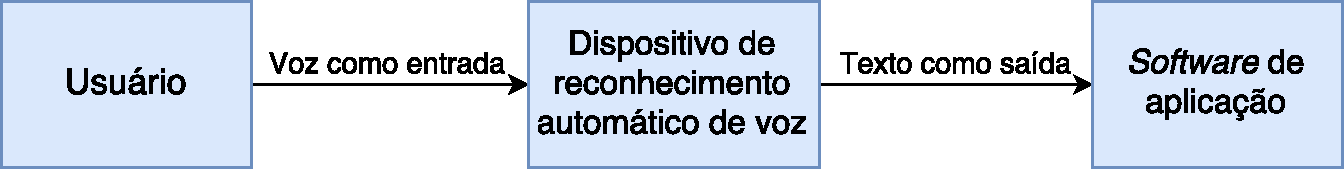
\includegraphics[width=.9\textwidth]{image/generic-stt.pdf}
  \caption{Sistema genérico de reconhecimento automático de voz}
  \label{generic-stt}
\end{figure}

% ---------------------------------------------------------------------

\section{História}

% https://nexbridge.co.uk/speech-recognition-in-the-21st-century/
% https://www.callcentrehelper.com/the-top-five-uses-of-speech-recognition-technology-1536.htm
% http://www.pcworld.com/article/243060/speech_recognition_through_the_decades_how_we_ended_up_with_siri.html
O primeiro sistema de reconhecimento de voz conhecido foi o \textit{Audrey}, construído em 1952 por três pesquisadores do \textit{Bell Labs} para reconhecer dígitos falados por um único usuário.

10 anos depois, a IBM apresentou o \textit{Shoebox}, que reconhecia 16 palavras em inglês, entre elas os dígitos de 0 a 9. Quando captava palavras como \textit{plus}, \textit{minus} ou \textit{total}, \textit{Shoebox} instruía outra máquina de adições a realizar cálculos ou imprimir o resultado. A entrada era feita por um microfone (figura \ref{shoebox}), que convertia a voz do usuário em impulsos elétricos, classificados internamente por um circuito de medição.


% Shoebox text: https://www-03.ibm.com/ibm/history/exhibits/specialprod1/specialprod1_7.html
% Image: http://www.cassiopeia.it/resources-2/computing-history-timeline/
\begin{figure}[H]
  \centering
  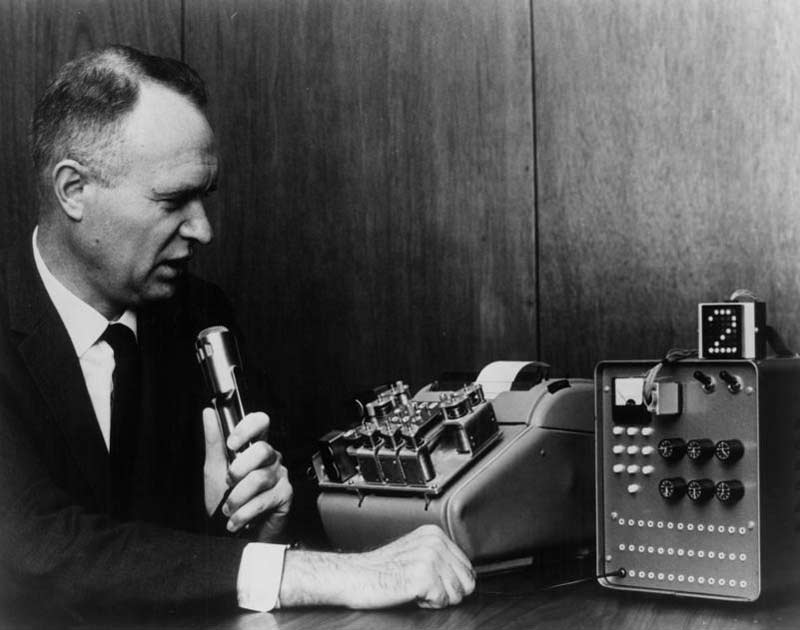
\includegraphics[width=.5\textwidth]{image/shoebox.jpg}
  \caption{Máquina \textit{Shoebox} sendo operada}
  \label{shoebox}
\end{figure}

Sistemas de reconhecimento de voz só tiveram um avanço realmente significativo na década de 80, devido a um método estatístico denominado \emph{modelo oculto de Markov} (ou \textbf{HMM}, sigla para \textit{Hidden Markov Model}). Ao invés de procurar por modelos de palavras em padrões de som, HMM considerava a probabilidade de um som desconhecido possuir palavras, o que acelerou o processo e tornou possível usar um vocabulário maior nos computadores. Outro modelo que ganhou bastante popularidade na época foi o de redes neurais, que é efetivo para classificar palavras isoladas e fonemas individuais mas encontra problemas em tarefas envolvendo reconhecimento contínuo. Ao contrário do HMM, este método não consegue modelar bem dependências temporais.

A evolução na tecnologia de reconhecimento de voz foi tamanha que, atualmente, é inegável seu impacto em nosso dia a dia. Um celular moderno consegue captar palavras ou pequenas frases de seu usuário dentre um enorme vocabulário para fazer buscas na Internet, tocar uma música ou fazer uma ligação. Muitas empresas utilizam máquinas para receber ligações de seus clientes; de acordo com o que interpretam, a chamada é redirecionada para um funcionário mais adequado. Alguns países chegam até a usar reconhecimento de voz para autenticar a identidade de alguém por telefone, com o objetivo de evitar fornecer dados pessoais pelo mesmo. Também há usos em transportes, na área médica e para fins educativos.

% ---------------------------------------------------------------------

\section{Parâmetros principais}

% https://www.nap.edu/read/19357/chapter/4#10
% http://www.voice-commands.com/103.htm
Há diversos tipos de parâmetros que caracterizam as capacidades de um sistema de reconhecimento de voz. Eles se subdividem nos três tipos a seguir.

% ---------------------------------------------------------------------

\subsection{Específicos ao aplicativo}

Estão relacionados à \emph{forma} com que o aplicativo em si realiza o reconhecimento de voz. Inclui dois parâmetros:

\begin{itemize}
\item A \textbf{forma de falar}, que pode ser através de \emph{palavras isoladas}, com pausas entre elas; \emph{palavras conectadas}, que são concatenadas sem pausas; ou \emph{fala contínua}, onde o fluxo de palavras é semelhante a uma fala natural.

\item \textbf{Existência de treinamento}, que subdivide aplicativos em dois grupos:

% https://speechangel.com/2016/05/04/difference-speaker-dependent-speaker-independent-recognition-software
\begin{itemize}[label=\scriptsize$\bullet$]
\item Os sistemas \textbf{dependentes} (\textit{speaker-dependent}), caracterizados pelo \emph{treinamento} feito pelo usuário. Isto é, são computadores que analisam e se adaptam aos padrões particulares da fala captada, resultando em uma maior acurácia. Geralmente, o usuário deve ler algumas páginas de texto para a máquina antes de começar a usar o sistema. Esta variante é comumente usada em casos particulares, onde um número limitado de palavras deve ser reconhecido com bastante precisão.

\item Os sistemas \textbf{independentes} (\textit{speaker-independent}), que são desenvolvidos para reconhecer a voz de qualquer pessoa e não requerem treinamento. É a melhor opção para aplicações interativas que usam voz, já que não é viável fazer com que os usuários leiam páginas de texto antes do uso. Sua desvantagem é a acurácia menor se comparado ao reconhecimento dependente; para contornar isso, costuma-se limitar o vocabulário reconhecido pelo sistema.
\end{itemize}

\end{itemize}

% ---------------------------------------------------------------------

\subsection{Específicos à tarefa}

Dependendo do objetivo a ser alcançado com o reconhecimento de voz, alguns parâmetros podem ser melhor ajustados para obter maior velocidade ou acurácia. São eles:

\begin{itemize}
\item O \textbf{vocabulário}, referente a quantas palavras são reconhecidas pelo sistema. O tamanho pode ser pequeno (menor que 20 palavras) até muito grande (mais de 20 mil palavras), sendo diretamente proporcional à velocidade do reconhecimento. Além disso, a similaridade entre a pronúncia de algumas palavras pode afetar a acurácia, uma vez que a distinção entre elas torna-se mais complicada.

\item A \textbf{sintaxe}, isto é, a gramática artificial que o sistema aceita para uma determinada tarefa. O exemplo mais simples seria uma máquina de estados finita, onde as palavras permitidas após um estado ou nó são definidas explicitamente.

\item O \textbf{fator de ramificação}, que é uma forma de medir a complexidade da sintaxe. É definido como o número médio de palavras permitidas em cada nó da gramática, e possui grande impacto sobre o desempenho do sistema.
\end{itemize}

% ---------------------------------------------------------------------

\subsection{Ambientais}

Dentre os vários parâmetros externos ao sistema e que podem interferir no reconhecimento de voz, destacam-se:

\begin{itemize}
\item A taxa \textbf{sinal-para-ruído}, que avalia a intensidade média do sinal recebido em relação ao ruído de fundo, tipicamente medido em decibéis (dB). Quanto menor a taxa, maior a dificuldade no reconhecimento de voz.

\item O \textbf{próprio usuário}, o que inclui o volume de sua voz, a velocidade com que fala e até mesmo sua condição psicológica: o nível de estresse de um piloto sob ataque em uma aeronave é diferente de alguém simplesmente querendo ouvir uma música, por exemplo.
\end{itemize}

% \chapter{Bibliotecas para Reconhecimento de Voz}
\label{cap:speech-libs}

A seguir, veremos o primeiro item necessário para atingirmos o objetivo final: uma biblioteca que fará o reconhecimento de voz dentro do módulo.

Uma implementação do zero fugiria do tema deste trabalho, pois seria necessário aprender sobre reconhecimento de padrões voltado a sons e outros tópicos relacionados a Inteligência Artificial. A outra opção existente, e a que seguiremos, é procurar por uma biblioteca existente e aprender a manejá-la.

Analisaremos quais as características necessárias e desejáveis na biblioteca ideal, e estudaremos a que melhor se adequa ao nosso objetivo dentre as opções existentes.

% ---------------------------------------------------------------------

\section{Considerações iniciais}

Recordemos os principais componentes para reconhecimento de voz, apresentados na seção \ref{sttComponents}. No contexto do módulo de reconhecimento de voz para \textit{Godot}, as seguintes associações surgem naturalmente:

\begin{itemize}
\item O \textbf{usuário} representa tipicamente o \textbf{jogador}, que interage parcialmente ou totalmente com o jogo por meio de comandos de voz.

\item O \textbf{dispositivo de STT} corresponde ao \textbf{módulo de reconhecimento de voz}, objetivo principal deste trabalho. Esta componente é usada pelo jogo para converter a fala do jogador em texto.

\item O \textbf{software de aplicação} é o \textbf{jogo} em si, feito em \textit{Godot}, que recebe indiretamente os comandos do usuário e realiza ações apropriadas.
\end{itemize}

% ---------------------------------------------------------------------

\section{A biblioteca ideal}
\label{idealLibrary}

Realçamos novamente que o módulo de reconhecimento de voz será usado diretamente em jogos. Tal contexto automaticamente nos leva a pensar em diversas características que a biblioteca ideal deve possuir.

% ---------------------------------------------------------------------

\subsection{Características obrigatórias}

Em ordem decrescente de importância, temos:

\begin{enumerate}
\item \textbf{Ter código aberto e licença permissiva:} Justifica-se pela integração da biblioteca em uma \textit{game engine} de código aberto. A importância é ainda maior se levarmos em conta que jogos com fins comerciais podem ser produzidos em \textit{Godot}.

\item \textbf{Ser eficiente (rápida):} Já foi mencionado que o módulo de reconhecimento de voz será usado em uma \textit{game engine}. Um jogo é um \textit{software} onde tipicamente a eficiência é de extrema importância, pois costuma envolver a renderização de cenas várias vezes por segundo. Devido a isso, surge a necessidade da biblioteca ser \emph{rápida} para não afetar negativamente a experiência do jogador.

\item \textbf{Reconhecer inglês:} O inglês possui presença constante em cenários de computação. Portanto, é a única língua que a biblioteca deve obrigatoriamente oferecer suporte.

\item \textbf{Não ser pesada:} Não é desejável ter uma biblioteca que ocupe muito espaço em disco (o que poderia aumentar o tamanho do jogo que a utiliza) e memória (aspecto relacionado diretamente à eficiência).
\end{enumerate}

% ---------------------------------------------------------------------

\subsection{Características desejáveis}

Em ordem decrescente de importância, temos:

\begin{enumerate}
\item \textbf{Ser multiplataforma:} \textit{Godot} possibilita exportar jogos para diferentes plataformas, dentre elas Windows, MacOS, Unix, Android e iOS \citep{godotDeployPlatforms}. Uma biblioteca que possa ser compatível com o maior número possível destes sistemas operacionais tornaria o módulo de reconhecimento de voz mais flexível para a produção de jogos em diferentes ambientes.

\item \textbf{Reconhecer diferentes línguas:} Apesar da obrigatoriedade do inglês, a possibilidade de usar diferentes línguas aumentaria a versatilidade do módulo. Tal característica é acentuada ao notarmos que muitos jogos, hoje em dia, oferecem a possibilidade de alterar a língua.

\item \textbf{Ser implementada em C/C++:} Conforme veremos na seção \ref{cap:godot}, \textit{Godot} possui toda a sua base escrita em C++, linguagem também usada para a criação de módulos. A implementação da biblioteca na mesma linguagem ajudaria a simplificar problemas de compatibilidade. Eventualmente, C também é uma opção viável por ser aceita pela linguagem sucessora.
\end{enumerate}

% ---------------------------------------------------------------------

\section{Bibliotecas viáveis}

Realizou-se uma pesquisa por bibliotecas de reconhecimento de voz que sigam o máximo de características possíveis propostas na seção \ref{idealLibrary}. O artigo \citep{sttLibs} sintetiza razoavelmente bem os resultados da busca. A seguir, destacamos as quatro bibliotecas mais notáveis encontradas:

\begin{itemize}
\item \textbf{Kaldi} \citep{kaldi}: É a biblioteca mais recente da lista, com seu código publicado em 2011. Escrita em C++, é tida como uma biblioteca para pesquisadores de reconhecimento de voz.

\item \textbf{CMUSphinx} \citep{cmusphinx}: Desenvolvida pela \textit{Carnegie Mellon University}, possui diversos pacotes para diferentes tarefas e aplicações. O pacote principal é escrito em Java. Existe também a variante \emph{Pocketsphinx}, com características interessantes para este trabalho: é escrita em C, possuindo maior velocidade e portabilidade que a biblioteca original.

\item \textbf{HTK} \citep{htk}: Desenvolvida pela \textit{Cambridge University Engineering Department}, HTK é uma sigla para \textit{Hidden Markov Model Toolkit}. É escrita em C, com novas versões sendo lançadas consistentemente.

\item \textbf{Simon} \citep{Simon}: Popular para Linux e escrita em C++, Simon utiliza \textit{CMUSphinx}, \textit{HTK} e \textit{Julius} internamente. Não havia suporte para \textit{MacOS} até abril de 2017.
\end{itemize}

% TODO: Explain better each library and the comparison article
Um artigo de 2014 comparou \emph{Kaldi}, \emph{CMUSphinx} e \emph{HTK} em relação a precisão e tempo gasto \citep{compareSpeech}. \emph{Kaldi} obteve resultados vastamente superiores; \emph{CMUSphinx} obteve bons resultados em pouco tempo; \emph{HTK} precisou de muito mais tempo e treino para conseguir resultados na ordem dos outros dois.

% ---------------------------------------------------------------------

\section{\textit{Pocketsphinx}, a biblioteca escolhida}

% TODO: Write this section


% ---------------------------------------------------------------------
% Appendix

% Header
\renewcommand{\chaptermark}[1]{\markboth{\MakeUppercase{\appendixname\ \thechapter}} {\MakeUppercase{#1}} }
\fancyhead[RE,LO]{}
\appendix

% Add appendix files here

% ---------------------------------------------------------------------
% Bibliography

\backmatter \onehalfspacing
\bibliographystyle{bib/plainnat-ime}  % Textual bibliographic quote

% Add bibliography files here
% \bibliography{bib/reference}

% ---------------------------------------------------------------------
% Index

% \index{TBP|see{periodicidade região codificante}}
% \index{DSP|see{processamento digital de sinais}}
% \index{STFT|see{transformada de Fourier de tempo reduzido}}
% \index{DFT|see{transformada discreta de Fourier}}
% \index{Fourier!transformada|see{transformada de Fourier}}

% \printindex  % imprime o índice remissivo no documento

% ---------------------------------------------------------------------

\end{document}
